\documentclass{standalone}
\usepackage{tikz}
\begin{document}
	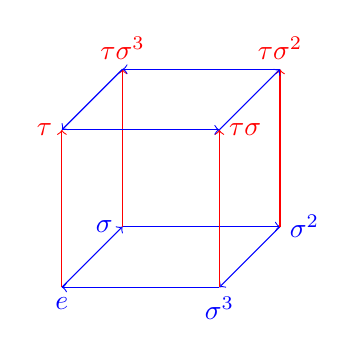
\begin{tikzpicture}
		\pgfmathsetmacro{\a}{2}
		\draw [blue,->] (0,0,\a) -- (0,0,0) node [left] {$\sigma$};
		\draw [blue,->] (0,0,0) -- (\a,0,0) node [right] {$\sigma^2$};
		\draw [blue,->] (\a,0,0) -- (\a,0,\a) node [below] {$\sigma^3$};
		\draw [blue,->] (\a,0,\a)-- (0,0,\a) node [below] {$e$};
		\draw [red,->] (0,0,\a) -- (0,\a,\a) node [left] {$\tau$};
		\draw [red,->] (\a,0,\a) -- (\a,\a,\a) node [right] {$\tau\sigma$};
		\draw [red,->] (\a,0,0) -- (\a,\a,0) node [above] {$\tau\sigma^2$};
		\draw [red,->] (0,0,0) -- (0,\a,0) node [above] {$\tau\sigma^3$};
		\draw [blue,->] (0,\a,\a) -- (\a,\a,\a);
		\draw [blue,->] (\a,\a,\a) -- (\a,\a,0);
		\draw [blue,->] (\a,\a,0) -- (0,\a,0);
		\draw [blue,->] (0,\a,0) -- (0,\a,\a);
	\end{tikzpicture}
\end{document}